\chapter{مرجع فارسی}\label{chp:chap4}
\thispagestyle{empty}
%===============================
\chapter{نحوه ی تولید فایل 
	\lr{bib}
	}
	
	برای نوشتن ارجاعات در متن و تهیه‌ی لیست ارجاعات نیاز به یک فایل با پسوند 
	\lr{.bib}	
	داریم. این فایل bib‌ بعدا در انتهای متن هنگامی که دستور 
\begin{latin}
\begin{lstlisting}[style=Tex]
\bibliography{biblographyFilename.bib}
\end{lstlisting}
\end{latin}
را وارد می کنیم تا لیست مراجع را برایمان تولید کند، مورد نیاز خواهد بود.
	
	نگران دستورات نباشید در قالب همه‌ی دستورات و تنظیمات قبلا نوشته شده‌اند و شما کافی است اطلاعات خودتان را به جای اطلاعات موجود وارد کنید.
	
	برای تولید فایل با پسوند bib دو راه وجود دارد. راه اول این است که این فایل را به صورت دستی تولید کنیم. راه دوم که راه بسیار بهتری است این است که از نرم افزار های موجود که این فایل را برای ما تولید می کنند استفاده کنیم. همانند کاری که غالبا دوستان با نرم افزار EndNote در word انجام می‌دهند. من اکیدا استفاده از روش دوم یعنی استفاده از نرم افزار را پیشنهاد می‌کنم. با این حال روش دستی را نیز برای کسانی که علاقه مند هستند توضیح می‌دهم.
	\section{تولید فایل به صورت دستی }
	برای تولید فایل به صورت دستی کافی است مطابق با الگوهای زیر عمل کنید. یک فایل درست کنید و  پسوند آن را به  bib تغییر دهید . توجه داشته باشید که در هنگام نامگذاری فایل ، اسم فایل نباید دارای فاصله باشد. اطلاعات مقاله‌ی مورد نظر را با الگوی زیر وارد کنید. به جای اطلاعات داخل کروشه اطلاعات مربوط به مقاله‌ی مورد نظر را وارد کنید. برای هر مرجع یک بار باید این فرم را در همان فایل bib کپی کنید و اطلاعات آن را وارد کنید. 
\begin{latin}
	\begin{lstlisting}[style=Tex]
@article{citekey1,
	author = {Family1, Name1 and Family2, Name2},
	doi = {doiAdress},
	journal = {Jurnal Name},
	pages = {Pages},
	title = {{Article title}},
	url = {http://ulr.url},
	volume = {Volume},
	year = {1992}
	}
\end{lstlisting}
\end{latin}
در مورد کتاب می توانید به شیوه ی زیر عمل کنید.
\begin{latin}
	\begin{lstlisting}[style=Tex]
@book{citekey2,
	author = {Family1, Name1 and Family2, Name2 },
	doi = {doi},
	edition = {edition},
	editor = {Editors},
	isbn = {ISBN},
	pages = {Pages},
	publisher = {Publisher},
	title = {{Book title}}
	}
	\end{lstlisting}
\end{latin}

توجه داشته باشید که نوشتن پر کردن همه ی اطلاعات فرم های بالا ضروری نیست و اطلاعاتی را که ندارید می‌توانید پاک کنید. درآخر هم فایل را ذخیره کنید.

در مورد مراجع فارسی تنها تفاوت یک کلید اضافه است که زبان را تعیین می کند از این  رو کلید \lr{language=persian} را باید در مدخل مورد نظر وارد کنیم. نمونه‌ای از این حالت در برایتان در ادامه آورده ام.
\begin{latin}
	\begin{lstlisting}[style=Tex]
@ARTICLE{Vahedi87,
  AUTHOR =  {%*\rl{  واحدی, مصطفی} *) },
  TITLE =  {%*\rl{ درختان پوشای کمینه دورنگی مسطح}*)},
  JOURNAL =  {%*\rl{مجله فارسی نمونه}*)},
  VOLUME =  {1},
  YEAR =  {1387},
  NUMBER =  {2},
  MONTH =  {%*\rl{آبان}*)},
  PAGES =  {22-30},
  doi = {10.1103/PB.47.1651},
  language =   {Persian}
}
	\end{lstlisting}
\end{latin}
	
\section{تولید فایل به وسیله ی نرم افزار}
برای تولید این فایل نرم افزار های زیادی وجود دارد. یکی از نرم افزار‌هایی که کار را بسیار راحت کرده است نرم افزار 
\lr{Mendaley Desktop}
است. این نرم افزار  رایگان است و بر روی همه ی  سیتم عامل ها چه ویندوز ، چه لینوکس یا مک و حتی بر روی اندروید قابل نصب است. توجه داشته باشید که با هر نرم افزاری که بتوانید با آن خروجی bib بگیرید قادر هستید کارهای مراجع پایان نامه‌ی خود را انجام دهید. نرم افزار mendeley علاوه بر قابلیت‌های نرم افزار‌های دیگر، قابلیت های زیر را نیز دارد:
\begin{itemize}
	\item مدیریت فایل‌های مقالات و دسته بندی آنها را انجام می دهد.
	\item تولید فایل \lr{.bib} که مورد نیاز برای لتکس است. البته با فرمت های دیگر که برای سایر برنامه‌ها مورد نیاز است نیز فایل خروجی تولید می کند.
	\item نرم افزار اطلاعات مقاله را از فایل \lr{PDF}  به صورت هوشمند یا با استفاده از اتصال به اینترنت و از منابع مقالات نظیر \lr{Science Direct} یا \lr{Google Scholar} استخراج می کند و این یعنی در انتهای کار احتمال این که اسم نویسنده ای را اشتباه وارد کرده باشید نیست و ارجاع مقاله به فرم صحیح وارد شده است.
	\item هماهنگ سازی منابع کتابخانه ای شما در صورتی که بیش از یک دستگاه برای مطالعه دارید را انجام می‌دهد فرض کنید که چند سیستم دارید یکی در دانشکده و یکی لبتاب شخصی خودتان و شاید حتی یک سیستم در خانه، با این برنامه نیازی نیست که هر بار تمامی مقالات و یا رفرنس های خود را در بین کامپیوتر‌های خودتان منتقل کنید. هر بار که یک مقاله یا فایل را در یکی از سیستم‌هایتان وارد کردید، آن فایل بر روی تمامی سیستم‌هایتان قابل دریافت است.
	\item  امکان Highlight کردن متون و جست و جو در متن مقالات و انتخاب متن آنها یا یادداشت گذاری در مقالات به نحوی که قابل جست و جو باشد نیز وجود دارد و همه ی اینها مجددا بر روی تمامی سیستم هایی که دارید قابل مشاهده است. 
	\item پیشنهاد مقالات جدید بر اساس مقالات موجود در کتابخانه با استفاده از ایمیل. نرم افزار به صورت اتوماتیک و در صورت تمایل در موضوعاتی که مقالات آن در کتابخانه‌تان موجود است، اگر مقاله‌ی جدیدی وارد شود به شما اطلاع می‌دهد و لینک آن را برایتان ارسال می کند.
	\item  قابلیت کار با word و تولید فرمت های مورد استفاده در EndNote و \lr{JabRef}. خود نرم افزار mendeley یک افزونه دارد که در word نصب می شود و با استفاده از آن می توانید در آن محیط هم کار مراجع را سامان بدهید.
\end{itemize}

برای دانلود 
\lr{Mendaley Desktop}
کافی است  به سایتش به آدرس 
\begin{latin}
	\url{https://www.mendeley.com/}
\end{latin}
مراجعه کنید و متناسب با سیستم عاملی که در اختیار دارید نسخه ی مناسب را دانلود کنید. 

برای استفاده از قابلیت های آن کافی است یک بار  در آن ثبت‌نام کنید.
\lr{Mendaley Desktop} 
یک افزونه هم دارد که بر روی مرورگرتان نصب می شود و هر جا که مقاله ای دیدید یا حتی ویدیو با سایتی که نیاز داشته باشید به آن ارجاع بدهید، با کلیک بر روی آن اطلاعات مربوط و لازم برای ارجاع دهی را به صورت خودکار و هوشمند دریافت می کند و به کتابخانه‌تان اضافه می‌کند.
برای نصب آن به آدرس زیر در محیط برنامه بروید 
\begin{latin}
	\begin{lstlisting}[style=Tex]
Tools --> Install Web Importer
	\end{lstlisting}
\end{latin}
\section{محیط برنامه }
\begin{figure}[h]
\centering
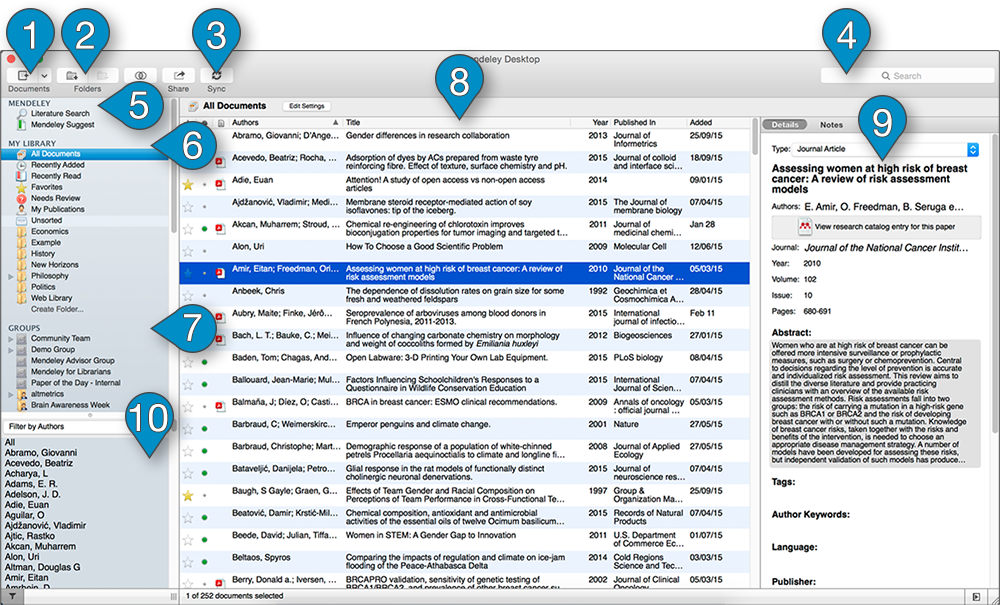
\includegraphics[width=\linewidth]{MDOverview}
\caption{شکل محیط برنامه}
\label{fig:MDOverview}
\end{figure}
به پیوست این قالب احتمالا دو فایل آموزش به صورت PDF قرار داده شده است که این نرم افزار رابه صورت کامل آموزش می‌دهند. با این حال اگر این دو فایل را نیافتید فقط کافی است به فارسی ``آموزش mendeley'' را جست و جو کنید. درضمن کتابخانه مرکزی دانشگاه هم، هر ترم دوره‌ی آموزشی این نرم‌افزار را برگزار می‌کند که خوب است شرکت کنید.
برای کسانی هم که علاقه‌مندند خودشان آموزش‌های اصلی را از سایت برنامه ببینند در آدرس زیر می‌توانند آموزش های مد نظرشان را پیدا‌کنند.
\begin{latin}
	\url{https://www.mendeley.com/guides/desktop/01-desktop-interface}
\end{latin}

فقط می ماند دو نکته که شاید به درد بخورد.

اول این که من معمولا مقاله را دانلود می کنم (به هر طریقی) بعد از آن با استفاده از 
\lr{Drag and Drop}
یا همان کشیدن و رها کردن خودمان فایل مقاله را به کتابخانه ی برنامه اضافه می کنم. حالا می‌ماند به دست آوردن مشخصات دقیق مقاله. اگر برنامه مشخصات دقیق را خودش پیدا کرده بود که هیچ، در غیر این صورت فقط کافی است 
\lr{doi}
مقاله را در قسمت 
doi
وارد کنیم و دکمه ی جست‌وجوی کنار آن را بزنیم، اطلاعات مربوط به مقاله از منابع معتبر دریافت می شود و در کتابخانه وارد می شود. 

کار وارد کردن منابع که تمام شد، آنهایی را که نیاز داریم انتخاب می کنیم. بر روی یکی از آنها کلیک راست می‌کنیم و بعد گزینه‌ی export‌ را انتخاب می‌کنیم. یک پنجره باز می شود که در آن آدرس فایل را برای ذخیره شدن انتخاب می کنیم. نام فایل را وارد می کنیم و کار تمام است. فقط حواستان باشد که نه تنها در اینجا بلکه در هیچ کجای لتکس نام هیچ فایلی را نباید با فاصله بنویسیم یعنی مثلا نباید بنویسید \lr{my biblography file name } باید همه‌ی اینها را سر‌هم بنویسید \lr{myBiblographyFileName}.

\section{نحوه‌ی ارجاع دهی در متن }
بعد از این که فایل با پسوند bib  را به هر نحوی تولید کردید نیاز است که در جاهای مختلف متن ارجاعات را مشخص کنید. اگر یادتان باشد آنجایی که داشتیم فایل bib را آماده می کردیم در ابتدای هر کدام از  ورودی ها یک عبارتی بود که من در مثال های بالا نام آنها را \lr{citekey1} و \lr{citekey2} گذاشتم. با استفاده از این کلید ها هر جای پایان نامه که باشد فرقی نمی کند (زیر عکس یا حتی در جدول ها و..) می توانید با نوشتن عبارت 
\begin{latin}
	\begin{lstlisting}[style=Tex]
\cite{citekey}
	\end{lstlisting}
\end{latin}
و آن کلید مربوطه مثلا citekey1 یا citekey2 در هر جای متن به آن مرجع به خصوص ارجاع دهید. 
در انتهای متن به صورت اتوماتیک و با تنظیمات مربوط به دانشگاه، لیست مراجع مرتب می شوند. 

\section{نحوه‌ی اجرای فایل لاتکس}
دانستن این نکته ضروری است که برای داشتن ترتیب مناسب مراجع نیاز است که لتکس را دو بار کامپایل کنید. حال اگر از برنامه های ویرایش متن خوبی نظیر texStudio استفاده می کنید، خود این برنامه‌ها این کار را برای شما اتوماتیک انجام می‌دهند و گرنه باید خودتان به این ترتیبی که می‌گویم فایل لتکس را کامپایل کنید.
\begin{enumerate}
	\item xelatex
	\item BibTex
	\item xelatex
	\item xelatex
\end{enumerate}
بار اول لتکس می فهمد که در اینجا یک سری رفرنس و مرجع وجود دارد. با اجرای مرحله‌ی دوم فایل‌های مربوط به مراجع را می‌خواند و آماده می‌کند. با اجرای مرحله ی سوم به هر مرجع در متن یک شماره می‌دهد و با اجرای مرحله‌ی چهارم این شماره‌ها را مرتب می‌کند. 
% =======================================================================
\section{ نمونه‌ هایی از مرجع زنی}\label{seq:4.1}
 در زیر نمونه‌هایی از مرجع زنی را می بینید.
 
 مرجع \cite{Vahedi87} یک نمونه مقاله مجله فارسی است.\\
مرجع \cite{Amintoosi87afzayesh}  یک نمونه  مقاله کنفرانس فارسی \\
مرجع \citep{Amintoosi87afzayesh}  یک نمونه  مقاله کنفرانس فارسی \\
نمونه ای از چند مرجع با هم \cite{Eschrig2003,Koepernik1997,Opahle1999}.